\chapter{Analisis dan Perancangan}

\section{Analisis Masalah}

Akan digunakan teknik parametrik neural untuk membangkitkan suara alat musik gesek. Untuk teknik ini, terdapat beberapa perbedaan masalah dengan penelitian sebelumnya\parencite{bonada2017singing}. Perbedaan masalah yang terjadi terdapat pada data input untuk sintesis, data latih, \textit{timing}, dan konteks.

Perbedaan masalah untuk data input sintesis terkait dengan \textit{timbre}. Dalam pembangkitan suara alat musik gesek, \textit{timbre} ditentukan oleh konteks. Hal ini berbeda dengan penelitian sebelumnya, di mana \textit{timbre} ditentukan dari rangkaian fonem yang terdapat dalam data input.

Perbedaan masalah terkait dengan data latih terdapat pada pewaktuan. Dalam penelitian ini, pewaktuan tidak terdapat pada data input.

\textit{Timing} not dalam alat musik gesek memiliki karakteristik yang berbeda dengan suara nyanyian. Dalam sistem baseline untuk suara nyanyian, terdapat \textit{timing} fonetik. Dalam sistem ini, tidak ada \textit{timing} fonetik. Hanya dibutuhkan \textit{timing} not saja.

Perbedaan masalah terkait konteks yaitu pada medan reseptif dari jaringan syaraf tiruan pada baseline. Baseline yang digunakan memiliki medan reseptif 100ms. Kecilnya medan reseptif ini berpengaruh kepada suara ekspresif secara umum, dan juga kepada penentuan \textit{timbre}. Untuk membangkitkan suara ekspresif, dibutuhkan konteks global dan konteks lokal dari not. Selain itu, konteks juga dibutuhkan dalam \textit{timbre}, yang dalam sintesis suara alat musik gesek tidak dipandu oleh rangkaian fonem.

\section{Rancangan Umum Sistem}

Untuk mengatasi masalah-masalah yang telah disebutkan, akan digunakan teknik neural parametrik serupa dengan baseline\parencite{bonada2017singing} dengan modifikasi. Modifikasi pertama yang diajukan adalah modifikasi pada arsitektur umum sistem. Modifikasi kedua yang diajukan dilakukan kepada arsitektur jaringan syaraf tiruan.

Arsitektur sistem yang diajukan terlihat pada gambar \ref{fig-system-overview}, sebagai modifikasi dari gambar \ref{fig-system-overview-bonada}. Dalam sistem ini, tidak ada masukan \textit{timing} fonetik untuk pelatihan. Partitur yang menjadi masukan pun tidak memiliki deskripsi fonem dan lirik. Model \textit{timing} fonetik diganti menjadi model \textit{timing}. Dalam sistem ini, ada komponen tambahan yaitu alignment dan analisis \textit{timing}.

Dalam sistem ini, \textit{timing} tidak diberikan dari data latih. Karenanya, \textit{timing} harus mampu diinferensi dari masukan partitur dan audio saja. Untuk inferensi \textit{timing} dari audio dan partitur, digunakan teknik alignment menggunakan masukan partitur dan hasil analisis vocoder dari audio. Hasil analisis vocoder yang digunakan adalah frekuensi fundamental dan kesunyian.

Berbeda dengan sistem baseline, model \textit{timbre} yang diajukan dalam sistem ini harus mampu menentukan \textit{timbre} dari konteks partitur. Karenanya, model \textit{timbre} dalam pelatihan menerima masukan partitur dan \textit{timing}, lalu dilatih untuk memprediksi data analisis vocoder. Parameter analisis vocoder yang diprediksi oleh model \textit{timbre} adalah spectral envelope dan komponen aperiodic.

Model \textit{timing} dalam sistem ini dilatih menggunakan partitur dan hasil analisis \textit{timing}. Dengan demikian, diharapkan model \textit{timing} dapat memprediksi \textit{timing} dari not dalam partitur.

Model pitch dalam sistem ini dilatih untuk menghasilkan F0. Masukan model ini adalah partitur dan \textit{timing}. Dalam pelatihan, masukan partitur diambil dari data latih, \textit{timing} diambil dari hasil alignment dan analisis \textit{timing}, dan parameter vocoder diambil dari hasil analisis vocoder terhadap audio.

Dengan demikian, terdapat tiga model, yaitu model \textit{timing}, \textit{pitch}, dan \textit{timbre}. Masukan dan keluaran tiap-tiap model ini tertulis dalam tabel \ref{tab-models-in-out}. Terdapat dua perbedaan dari masukan dan keluaran model-model baseline pada tabel \ref{tab-models-in-out-bonada}. Pertama, tidak ada fonetik. Kedua, model \textit{timbre} menerima masukan partitur.

\begin{table}[h]
    \centering
    \caption{Masukan dan Keluaran Tiap Model dalam Sistem Sintesis Parametrik Neural Suara Alat Musik Gesek }\label{tab-models-in-out}
    \begin{tabular}{ |c|c|c| } 
     \hline
     Model & Masukan & Keluaran \\
     \hline 
     Model \textit{timing} & partitur & \textit{timing} not (dengan penyimpangan) \\ 
     \hline
     Model \textit{pitch} & partitur & F0 \\ 
      & \textit{timing} (terdistorsi) not  & \\ 
     \hline
     Model \textit{timbre} & partitur & V/UV \\ 
      & \textit{timing} (terdistorsi not)  & Komponen harmonik\\ 
      & F0  & Komponen aperiodisitas\\ 
     \hline
    \end{tabular}
\end{table}

\begin{figure}[h]
    \centering
    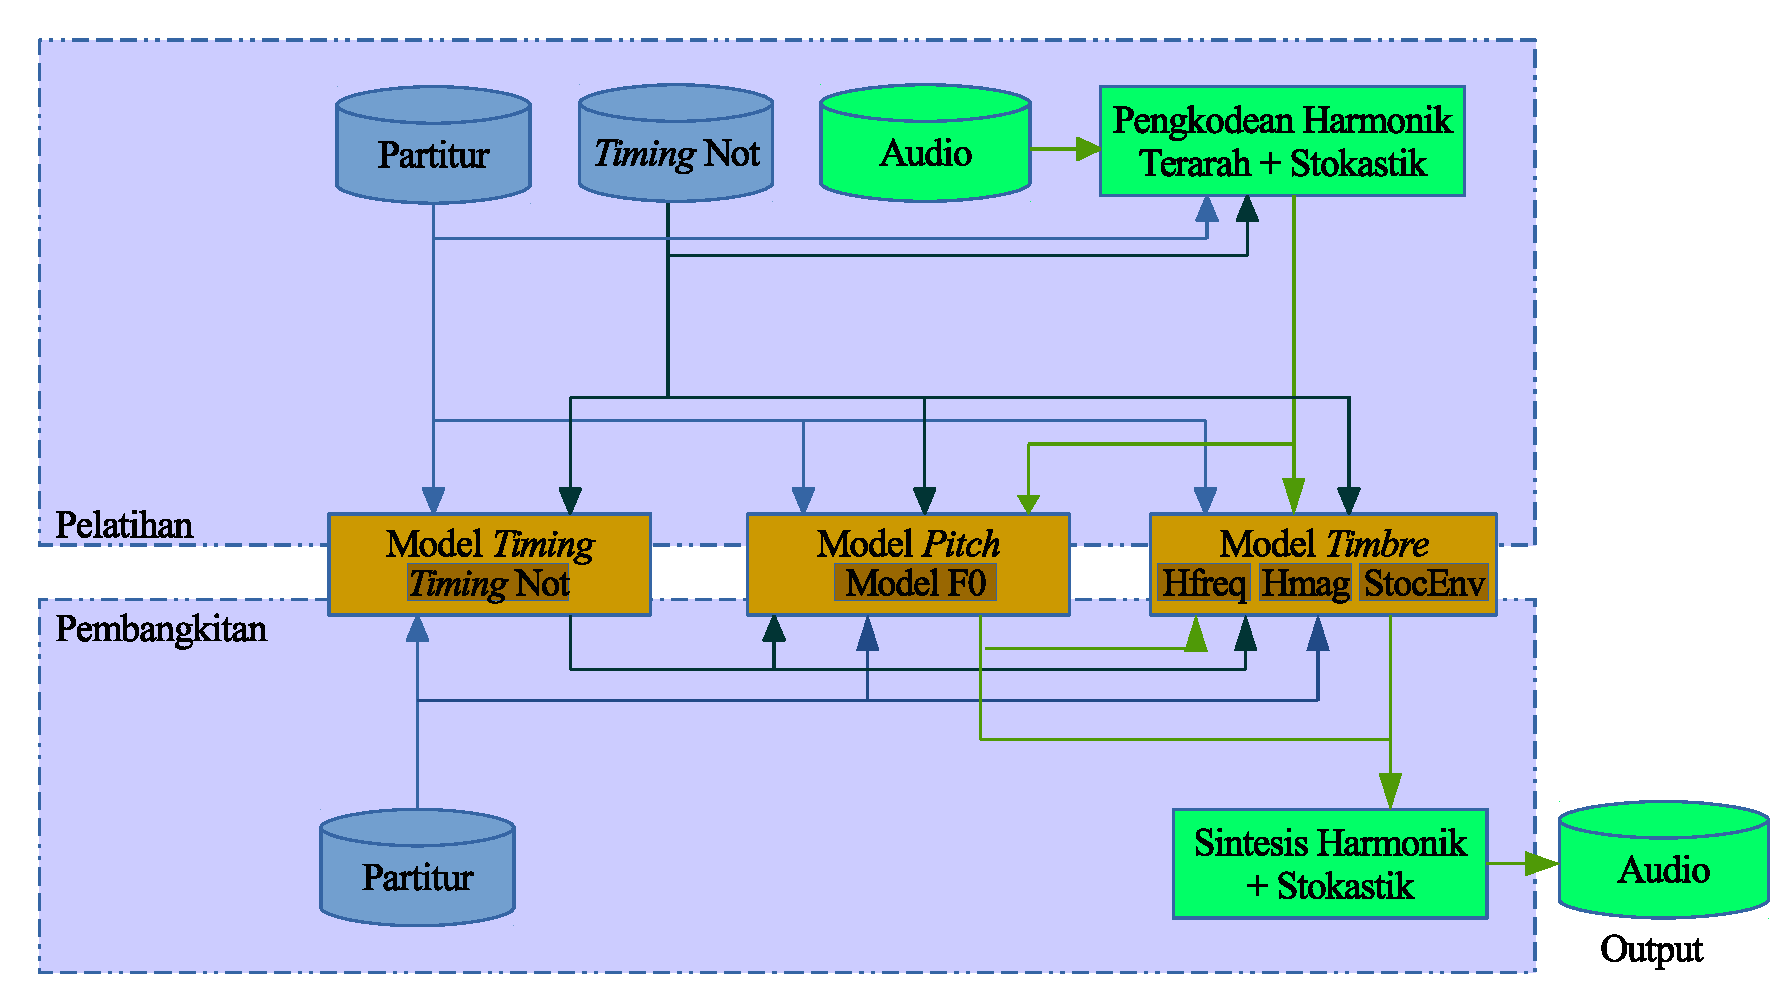
\includegraphics[width=0.8\textwidth]{resources/system-overview.eps}
    \caption{Arsitektur sistem permainan musik ekspresif alat musik gesek yang diajukan (modifikasi gambar \ref{fig-system-overview-bonada})}\label{fig-system-overview}
\end{figure}

Pada tahap pembangkitan, sistem ini mampu menerima partitur dan menghasilkan audio. Keluaran perantara yang dihasilkan adalah parameter vocoder, yang kemudian digunakan oleh vocoder untuk menghasilkan audio.

Hal pertama yang dilakukan dalam tahap pembangkitan adalah prediksi \textit{timing} not. Setelah itu, partitur dan \textit{timing} not digunakan untuk memprediksi pitch an \textit{timbre}, dengan model yang sesuai. Parameter pitch -frekuensi fundamental- dan parameter \textit{timbre} -spectral envelope dan aperiodisitas- digunakan untuk sintesis vocoder.

Tiap model dari model-model ini adalah model regresi. Untuk model \textit{timing}, digunakan jaringan syaraf tiruan \textit{feedforward}. Untuk model \textit{pitch} dan model \textit{timbre}, digunakan jaringan syaraf tiruan konvolusional terdilasi dengan elemen rekuren. Masukan dari jaringan syaraf tiruan ini terdiri dari masukan rekuren -output pada waktu sebelumnya- dan masukan kontrol.

Masukan kontrol jaringan syaraf tiruan ini berasal dari partitur dan dari \textit{timing}. Untuk model \textit{timing}, masukan kontrol hanya berasal dari partitur. Untuk model pitch dan model \textit{timbre}, masukan kontrol berasal dari partitur dan berasal dari \textit{timing}.

Masukan dari partitur dapat menunjukkan kondisi sesaat dan konteks. Kondisi sesaat berupa pitch asli, panjang not, dan waktu dalam not. Kondisi konteks dapat berupa not sebelum dan sesudah, interval, ataupun kondisi-kondisi lainnya hasil analisis karya. Namun, kakas analisis karya mungkin tidak akan digunakan karena riset terkait analisis karya menggunakan komputer masih minim.

\begin{figure}[h]
    \centering
    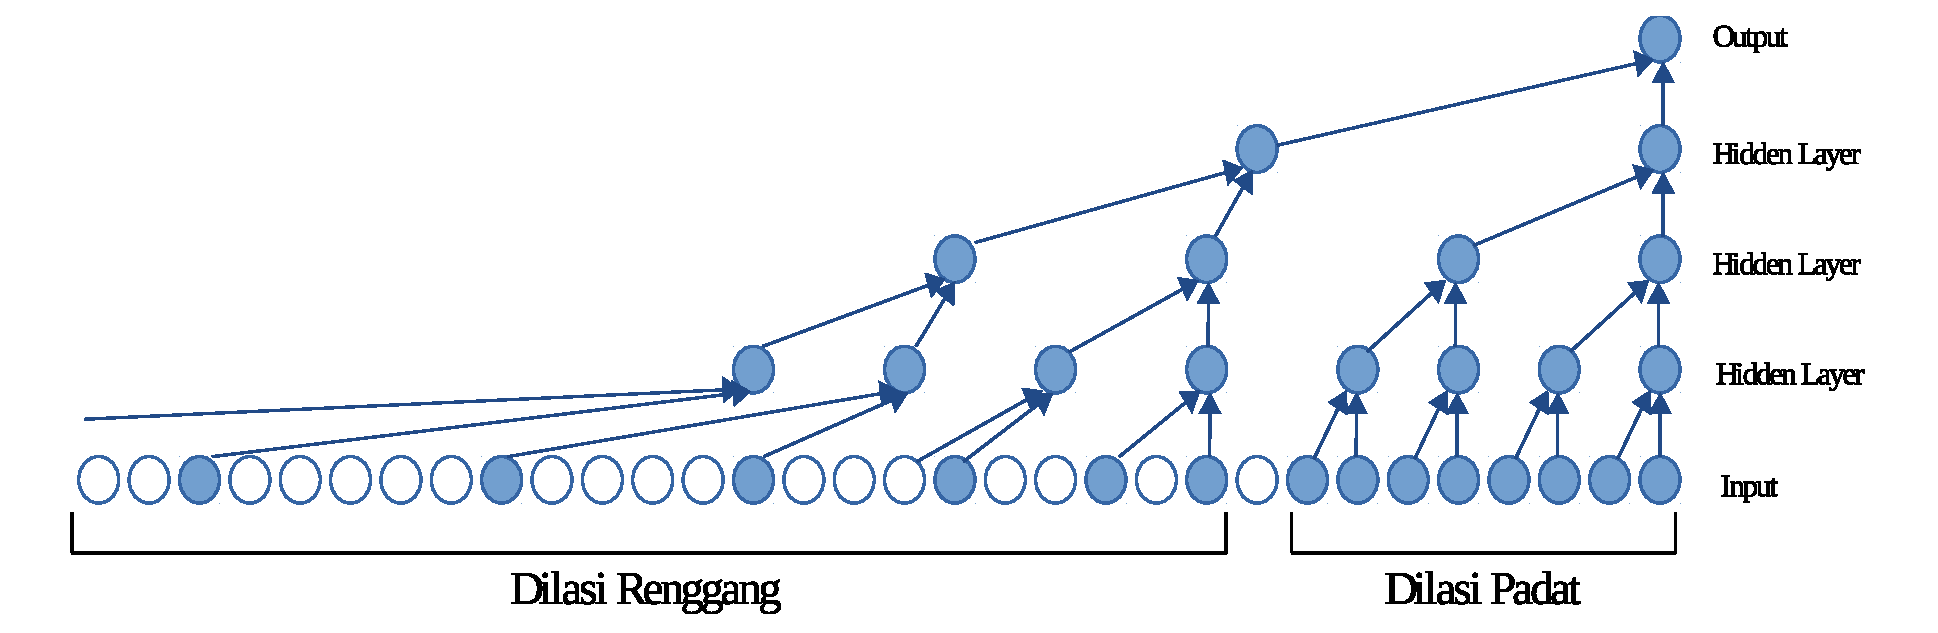
\includegraphics[width=0.8\textwidth]{resources/sparse-dense-dilated-cnn.eps}
    \caption{Arsitektur jaringan syaraf tiruan konvolusional dengan dilasi jarang-padat (modifikasi arsitektur pada gambar \ref{fig-dilated-cnn})}\label{fig-sparsedilated-cnn}
\end{figure}

Untuk mengatasi masalah medan reseptif dari model baseline, diajukan dilasi jarang-padat. Arsitektur jaringan syaraf tiruan yang merupakan modifikasi arsitektur pada gambar \ref{fig-dilated-cnn} terlihat pada gambar \ref{fig-sparsedilated-cnn}. Untuk simpul-simpul masukan yang dekat dengan frame yang sedang dibangkitkan, digunakan faktor dilasi sedemikian hingga semua simpul terlingkupi. Untuk simpul-simpul masukan yang jauh dari frame yang sedang dibangkitkan, digunakan faktor dilasi yang lebih besar. Dengan demikian, medan reseptif dapat ditingkatkan tanpa menambah jumlah simpul tersembunyi dan ukuran vektor bobot yang diestimasi.

Pada bagian dengan dilasi jarang, ada simpul-simpul yang dilewat. Dalam permasalahan suara alat musik gesek, hal ini tidak menjadi masalah. Karakteristik suara yang menjadi masukan rekuren banyak redundan. Adapun masukan kontrol untuk simpul-simpul yang berdekatan akan sama karena satu not dapat menjadi banyak frame di mana tiap frame menjadi simpul masukan.

Untuk melatih sistem ini, dibutuhkan data latih berupa partitur dan rekaman audio. Data yang dibutuhkan adalah data berpasangan. Detil pengumpulan data latih ini dijelaskan dalam subbab selanjutnya.

\section{Tahapan Pembangunan Sistem}

Terdapat empat tahapan pembangunan sistem:

\begin{enumerate}
    \item Pengumpulan data
    \item Implementasi program untuk pelatihan dan pembangkitan
    \item Pelatihan model
    \item Pengujian
\end{enumerate}

Pada tahap pengumpulan data yang dibutuhkan berupa data latih dan data uji. Dalam pengumpulan, data akan dihimpun menjadi satu kumpulan data. Kumpulan data tersebut akan dipisahkan menjadi data latih dan data uji setelah pengumpulan data selesai.

Untuk pengumpulan data, akan dicari partitur dan rekaman audio yang telah terpublikasi. Akan disaring instans data yang memiliki pasangan yang sesuai. Data rekaman audio tanpa partitur atau data partitur tanpa audio tidak akan dimasukkan kepada kumpulan data akhir. Kemudian, penyalin akan mendengarkan rekaman audio dan mencocokkan dengan partitur untuk memastikan bahwa rekaman audio sesuai dengan partitur. Partitur yang dikumpulkan akan disalin/dikonversi menjadi format teks (MusicXML/MIDI).

Karena pengujian yang akan dilakukan adalah pengujian pendengar manusia, data uji yang dibutuhkan berukuran kecil. Pemisahan data uji dari data latih dilakukan secara acak. Data uji akan diambil sejumlah 3-5 karya.

Implementasi program untuk pelatihan dan pembangkitan dilakukan menggunakan kakas-kakas \textit{vocoder} dan jaringan syaraf tiruan. Kakas jaringan syaraf tiruan yang digunakan adalah kakas yang mendukung jaringan syaraf tiruan \textit{feedforward}, konvolusi, dilasi, dan elemen rekuren. Hasil implementasi ini dapat digunakan untuk melatih model, yang kemudian digunakan untuk membangkitkan suara untuk diujikan kepada pendengar manusia.